\chapter{Introduction}\label{chap: intro}


\section{Bose-Einstein condensates}
The first theoretical prediction of Bose-Einstein condensation occurred in 1924,
when Indian physicist Satyendra Nath Bose, by re-deriving Planck's law of
black-body radiation, developed a theory of statistical mechanics of photons
by treating them as a collection of particles~\cite{Bose1924}.
Einstein firstly helped Bose publish his work, before later going on to
generalise the theory by applying it to a system of \(N\)-interacting
bosons~\cite{Einstein1925}.
This then led to the Bose-Einstein distribution, which describes the
statistics of bosons over single-particle energy states:
\begin{equation}\label{eq: Bose-Einstein-distribution}
    f(\epsilon_i) = \frac{1}{e^{(\epsilon_i-\mu)/k_B T} - 1},
\end{equation}
where \(\epsilon_i\) is the energy of level \(i\), \(\mu \) is the chemical
potential, \(k_B\) is the Boltzmann constant, and \(T\) is the temperature.

Since the total number of particles is conserved, the chemical potential enters
the above distribution.
The chemical potential itself is calculated from the total particle number \(N\)
and \(T\) by the condition that the total number of particles be equal to the
sum of the particles in the individual levels.
Mathematically, \(N\) is written as
\begin{equation}
    N = \sum_i N_i = \sum_i g(\epsilon_i)f(\epsilon_i),
\end{equation}
where \(N_i\) gives the mean occupation of level \(i\) and \(g(\epsilon_i)\)
gives the degeneracy of level \(i\) (i.e., the number of distinct states with
energy level \(\epsilon_i\)).

As \(T \rightarrow 0\), Eq.~\eqref{eq: Bose-Einstein-distribution} diverges,
which implies that the total excited state capacity has to decrease to keep
the number of particles fixed.
At the precise point where the total excited states cannot accommodate the total
number of particles, Bose-Einstein condensation occurs.
At \(T=0\), all atoms must occupy the lowest energy level of the system, called
the ground state.

\subsection{Transition temperature}
The critical temperature at which Bose-Einstein condensation occurs can be
derived as follows.
Let us consider a system of non-interacting bosons at thermal equilibrium at
temperature \(T\).
According to de Broglie, particles behave like waves and as such have an
associated wavelength termed the de Broglie wavelength.
This wavelength characterises the length scale of the particles localised
wave packet, and is conventionally written as
\begin{equation}\label{eq: de-Broglie-wavelength}
    \lambda_\text{dB} = \frac{h}{\sqrt{2\pi mk_B T}},
\end{equation}
where \(h\) is Planck's constant and \(m\) is the mass of the particle.
Since \(\lambda_\text{dB} \propto 1 / \sqrt{T}\), high temperatures
(\(T > T_c\)) imply that the de Broglie wavelength is small compared to the
average inter-particle spacing.
In this limit, the system exhibits classical, particle-like behaviour and the
particles closely follow the Boltzmann distribution.
Conversely, as the temperature decreases, the de Broglie wavelength associated
with each particle grows.
At some critical temperature, \(T_c\), the wavelengths of each particle become
comparable to the average inter-particle spacing and as such individual
particles become indistinguishable.
At this point the system exhibits quantum behaviour, and the particles form a
degenerate gas.

Assuming a uniform, three-dimensional system with volume \(\mathcal{V}\) and
number density \(N/\mathcal{V}\), the Bose-Einstein transition occurs when
\(n\lambda_{\text{dB}}^3 \leq \zeta(3/2)\)~\cite{Pethick2008}, where
\(\zeta \) is the Riemann zeta function.
Substituting in Eq.~\eqref{eq: de-Broglie-wavelength}, we find the critical
temperature for Bose-Einstein condensation:
\begin{equation}
    T_c = \frac{h^2}{2\pi mk_B}{\left(\frac{n}{\zeta(3/2)}\right)}^{2/3}.
\end{equation}

\subsection{Experimental realisation}
Alkali atoms, such as rubidium and sodium, present ideal candidates
for Bose-Einstein condensate experiments due to being weakly-interacting, easily
trapped magnetically, and their ability to be cooled using laser techniques.
Cooling such atoms, however, can lead to a transition into a liquid or a solid.
To prevent this, it is necessary to reduce the atomic density of the gas such
that elastic, binary collisions dominate.
Typical required densities for this to hold are around \(n \sim 10^{-14}
\text{cm}^3\).
Using the estimate for the critical temperature derived above, one can then
estimate that Bose-Einstein condensation would occur at \(T_c \sim 10^{-6}\)K
for such a system.

The first experimental realisations of Bose-Einstein condensates (BECs) occurred
in 1995, where the groups at JILA~\cite{Anderson1995}, MIT~\cite{Davis1995}, and
Rice University~\cite{Bradley1995} successfully cooled atoms of \(^{87}\)Rb,
\(^{23}\)Na, and \(^{7}\)Li, respectively, observing Bose-Einstein condensation.
For their pioneering work on ``the achievement of Bose-Einstein condensation in
dilute gases of alkali atoms, and for early fundamental studies of the
properties of the condensates'', Carl Wieman, Eric Cornell, and Wolfgang
Ketterle earned the 2001 Nobel Prize in Physics.
These works gave birth to a whole new field of research, and today, interest in
BECs has only accelerated further, with applications of such condensates ranging
from precision measurements~\cite{Obrecht2007} to quantum
computing~\cite{Byrnes2012}.

\subsection{Spin degree of freedom: Spinor Bose-Einstein condensates}
In experiments, a consequence of strong magnetic trapping of the atoms is the
``freezing'' of the atoms spin, where such condensates are referred to as
scalar (or spinless).
However, atomic spin, usually denoted as \(f\), need not be constrained, and
can instead become a degree of freedom within the system.
Experimentally, this is typically achieved through the use of optical trapping
potentials, which utilise the AC-Stark shift of atom to form a conservative
potential that traps all the Zeeman sublevels equally.
In this case, atoms can Bose-condense into each of the available component spin
states, \(m_F\), producing a multi-component condensate.
Such a condensate is called a spinor Bose-Einstein condensate, and forms the
main interest of this thesis.

The first experimental realisation of a spinor BEC occurred just three years
after the pioneering work in scalar systems, where, in 1998, a group at MIT
successfully produced a spin-1 condensate of \({^{23}}\)Na
atoms~\cite{Stamper-Kurn1998}.
Around the same time, seminal theory works by Ho~\cite{Ho1998} and Ohmi and
Machida~\cite{Ohmi1998} were developed, which kickstarted a new wave of research
into spinor BEC systems.
Advances in optical trapping and laser cooling since then have led to the
formation of spinor condensates in spin-1 and spin-2
\(^{87}\)Rb~\cite{Barrett2001, Schmaljohann2004},
spin-2 \(^{23}\)Na~\cite{Gorlitz2003}, and
even spin-3 \(^{52}\)Cr~\cite{Beaufils2008}.


\section{Topological defects in Bose-Einstein condensates}
Atomic BECs can support various topological excitations: Objects that are free
to move in space and time without changing their characteristics that are
defined by topological charges.
An example that arises in scalar BECs is the quantum phase vortex, a singular
line defect which carries mass circulation.
The first experimental realisation of a quantum vortex in an atomic BEC occurred
in 1999~\cite{Matthews1999}, which was achieved in a two-component \(^{87}\)Rb
condensate.
The process of generating the vortex was based on imparting angular momentum
to the condensate by rotating the trap in which it was held~\cite{Williams1999}.
However, instead of rotating the trap, a laser was instead focused on a small
region outside the condensate and rotated through a circular path.
Images taken from the experiment are shown in Fig.~\ref{subfig: first-vortex}.
\begin{figure}
    \centering
    \begin{subfigure}{0.49\textwidth}
        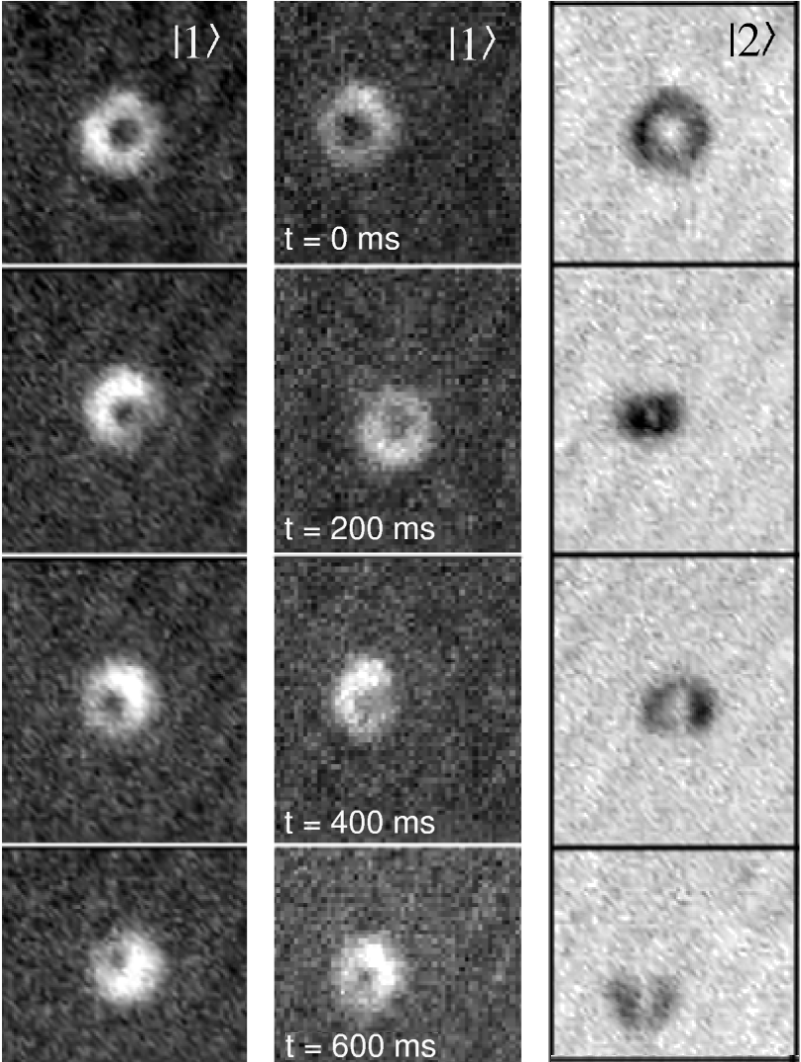
\includegraphics[width=\textwidth]
        {gfx/ch-introduction/first_quantum_vortex.png}
        \caption{\label{subfig: first-vortex}}
    \end{subfigure}
    \begin{subfigure}{0.49\textwidth}
        \centering
        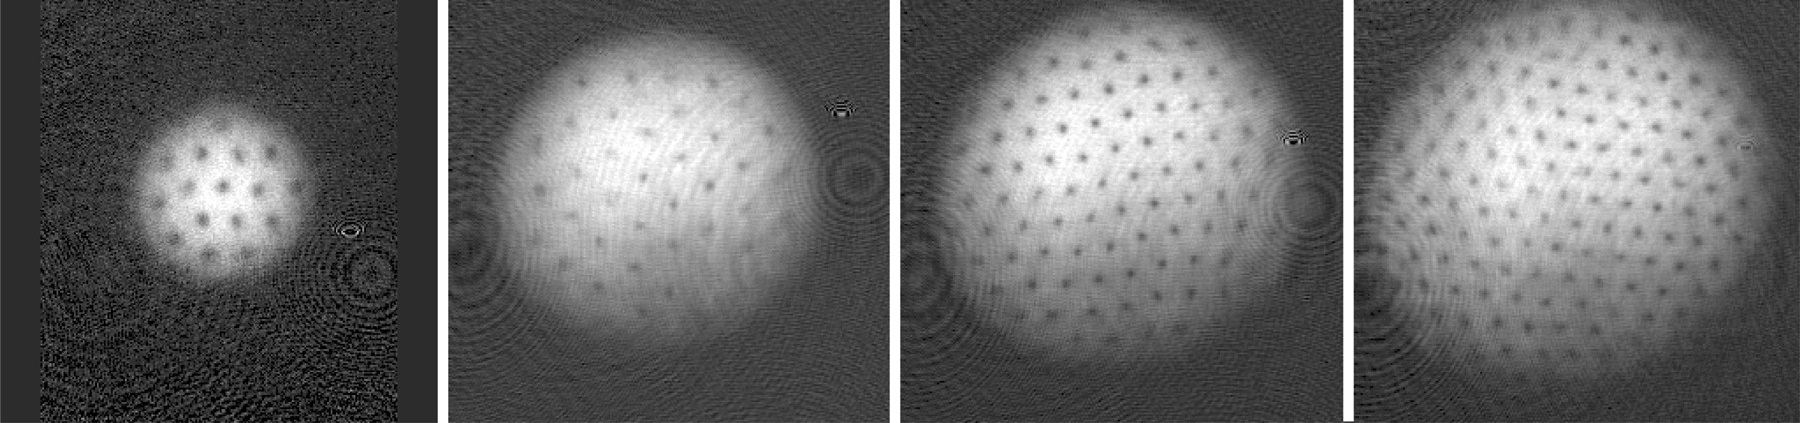
\includegraphics[width=1.32\textwidth, height=0.5\textwidth, angle=-90]
        {gfx/ch-introduction/vortex_lattice.jpeg}
        \caption{\label{subfig: vortex-lattice}}
    \end{subfigure}
    \caption[Experimental images of quantum vortices in atomic BECs]
    {Experimental images of quantum vortices in atomic BECs.
        (a): First experimental realisation of a quantum vortex in an atomic BEC,
        reproduced from Ref.~\cite{Matthews1999}.
        (b): Quantum vortex lattice, reproduced from Ref.~\cite{Abo-Shaeer2001}.
    }
\end{figure}
Further theoretical work generalised this idea by allowing the amplitude of the
rotating laser to spatially vary instead of being confined to a
point~\cite{Ruostekoski2000}.

Advances in experimental techniques led to the development of so-called stirring
lasers, where an incident microwave field applied to the condensate causes
it to stretch in the direction of the applied field.
Vortices could then be produced dynamically from the edge of the rotating trap
due to the slight asymmetries induced by the stirring laser.
These advances led to the formation of the first vortices within scalar
condensates~\cite{Madison2000, Madison2000a, Abo-Shaeer2001}.
Interestingly, rather than forming a single vortex with large angular momentum,
vortices constructed in this way form vortex lattices, i.e., the condensate
comprises many individual vortices of small angular momentum (see
Fig.~\ref{subfig: vortex-lattice}).

A system containing many vortices, sometimes referred to as a vortex tangle
in 3D systems, gives rise to a turbulent flow called quantum turbulence.
Due to their accessibility, quantum turbulence in atomic BECs has attracted
considerable theoretical~\cite{Kobayashi2007,Numasato2010, Reeves2013,
Billam2014,Simula2014,Baggaley2018} and experimental~\cite{Henn2009,Kwon2014,
Seo2017,Navon2019,Gauthier2019,Johnstone2019} attention.
Due to their richer family of topological defects, spinor and pseudospin-1/2
systems present a new avenue for studying the properties of quantum turbulence
and nonequilibrium dynamics~\cite{Salman2009, Schmied2019, Karl2013, Prufer2018,
Hofmann2014}.
In two-component condensates, when atomic mass and mean density of the
components are equal, vortices may arise which are characterise by a phase
winding in only one of the components, leading to what are known as half-quantum
vortices (HQVs) due to their similarities with vortices carrying half a quantum
of superfluid circulation in both \(^3\)He~\cite{Autti2016} and
spin-1 BECs~\cite{Leonhardt2000, Seo2015}.
These vortices have very different dynamics to scalar vortices arising in scalar
BECs, and cannot be described by simple point-vortex models~\cite{Eto2011,
Kasamatsu2016}.
Chapter~\ref{chap: two-comp} is dedicated to the study of a 2D system filled
with HQVs undergoing quantum turbulence.

The combination of a macroscopic condensate phase together with spin rotations
leads to an even richer phenomenology of topological defects present within
spinor BECs that are otherwise unseen in scalar and two-component condensates.
The existence and type of topological defects allowed within spinor BECs can be
found from the topology of the ground state manifold, and detailed constructions
of some topological defects present within these systems
are available in Chapter~\ref{chap: ground-states}.
Vortices, for example, are rich and varied in their characteristics within
spinor BECs.
Some examples are: Fractional vortices, which carry circulation in fractional
units compared to vortices arising in scalar condensates, spin vortices,
carrying a circulation of the condensate spin only, and nonsingular vortices,
textures that carry mass and/or spin circulation.
The existence of such vortices, however, does not imply their stability, and
many numerical studies have investigated the energetic stability of both
singular and nonsingular vortices in spinor condensates~\cite{Isoshima2001,
Mizushima2002, Mizushima2002a,Takahashi2009, Lovegrove2012, Lovegrove2014,
Lovegrove2016}.

Since the expanded order parameter space of spinor BECs allows for a variety of
different vortex states, including both singular and nonsingular vortices, if
one applies a stirring laser to such a condensate to nucleate vortices then it
is not always clear which types of vortices will nucleate.
Thus, instead of stirring lasers, other experimental techniques exist for
generating specific types of vortices in spinor systems.
For example, a nonsingular vortex was generated in a spin-1 \(^{23}\)Na
condensate by methods of phase-imprinting~\cite{Leanhardt2003}, where the
magnetic field bias was adiabatically reduced to zero along the trap axis.
This distributed the atomic population across the three internal spin states,
producing the required coreless spin texture.
The same technique was used to realise both singly- and doubly-quantised
vortices in a spin-polarised BEC, the latter of which was observed to undergo a
splitting process into two singly quantised vortices~\cite{Leanhardt2002,
Shin2004}.
More recently, experimental techniques have been developed that allow for the
controlled creation of vortices with internal point-group
symmetries~\cite{Xiao2022}, further opening up experimental accessibility for
investigating the unique properties of topological defects in spinor BECs.

Owing to their accessibility and high controllability, spinor BECs are also
excellent candidates for studying a range of nonequilibrium
physics~\cite{Schmaljohann2004}, including
relaxation dynamics~\cite{Gring2012, Reeves2022} and quantum
quenches~\cite{Sadler2006,Barnett2011,Navon2015,Symes2017,Kang2017,Prufer2018,
Schmied2019,Liu2020}.
By continuously changing an external parameter, such as the linear or quadratic
Zeeman shifts (see Sec.~\ref{subsec: single-particle}) through the use of
applied magnetic fields, the system can be ramped across a
quantum critical point~\cite{Sachdev2011} and undergo a quantum phase
transition.
Such a transition is defined as continuous (discontinuous) depending on whether
the derivative of the system energy with respect to the changing external
parameter is also continuous (discontinuous).
Spinor BECs posses a number of both continuous and discontinuous quantum
critical points between their ground state phases, making them an ideal test bed
for studying both types of quantum phase transitions.
An example of a second-order (continuous) quantum phase transition arises
between the polar and broken-axisymmetry phases in spin-1 BECs (see
Chapter~\ref{chap: ground-states}).
Naturally, they also make excellent candidates for investigating the
Kibble-Zurek mechanism (KZM), which governs the observed scaling laws when the
symmetry of a system is spontaneously broken after undergoing a continuous phase
transition~\cite{DelCampo2014}.
Much theoretical and experimental work has already confirmed Kibble-Zurek
scaling in a multitude of continuous quantum phase transitions in spinor
condensates~\cite{Sadler2006, Damski2006,Damski2007, Lamacraft2007,Saito2007,
Saito2007a,Vengalattore2008, Swislocki2013, Witkowska2013, Anquez2016,
Williamson2016,Kang2017}.
Furthermore, there has been the first experimental evidence of observed scaling
laws across a discontinuous quantum phase transition in a spinor
BEC~\cite{Qiu2020}, showing their excellent eligibility for studying the
lesser-known scaling laws associated with discontinuous phase transitions.

\subsection{Topological interfaces}
When a system contains multiple topologically distinct phases described by
different order parameters, a topological interface may form between them.
Such interfaces already arise in many areas of physics, from the context of
domains walls in the early universe~\cite{Zeldovich1975,Kibble1976,Kibble1980}
to the \(A\)--\(B\) phase boundary in superfluid liquid \(^3\)He~\cite{
Osheroff1977,Yip1986,Salomaa1987,Finne2006,Bradley2008,Volovik2009}.
The different bulk regions may also harbour topological defects, which either
terminate on the interface or smoothly connect to a topologically distinct
object on the other side.
Due to their rich phase diagram exhibiting a range of symmetries and defects,
spinor BECs provide an ideal testing ground for investigating topological
interface physics in a highly-controllable system.

Topological interfaces in spin-1 systems can be engineered through spatial
control of Zeeman shifts~\cite{Borgh2012, Borgh2013, Borgh2014}, leading to
a condensate containing two topologically distinct bulk regions described by
different symmetries.
In~\cite{Borgh2012}, a topological interface was formed between the polar and
ferromagnetic phases of a spin-1 BEC, and a range of topological defects were
constructed.
These defects ranged from simple singly-quantised vortices in both phases
connecting across the interface, to the more complicated case of HQVs in the
polar phase connecting to nonsingular vortices in the ferromagnetic phase, which
may even exist together with monopoles.
Interfaces may also form within vortex cores, where the bulk order parameter
outside the core continuously transforms into a different symmetry within
the core.
Such interfaces have already been experimental created in
spin-1~\cite{Weiss2019,Xiao2021} and spin-2~\cite{Xiao2022} BECs.
Their even richer phase diagram and family of defects implies that spin-2
condensates offer an even greater avenue of study for topological interface
physics.
They additionally have ground state phases with discrete polytope point-group
symmetries~\cite{Xiao2022,Semenoff2007,Yip2007,Kawaguchi2011} in which the
defects are non-Abelian~\cite{Mermin1979} and hence are dependent on other
defects within the system, leading to intriguing interface physics.

\section{Outline of the thesis}
An outline of the structure of this thesis and a description of each chapter is
given in this section.
The thesis is split into three main parts: Part I introduces the mathematical
models required to understand atomic BECs, and introduces the ground states,
symmetries, and topological defects present in spin-1 and spin-2 BECs.
Part II presents analytical and numerical work carried out to investigate
various areas of physics in spinor and pseudospin-1/2 condensates.
In particular, we cover three main areas: relaxation dynamics, discontinuous
quantum phase transitions, and topological interfaces.
Finally, part III is a collection of appendices relating to numerical methods
or detailed derivations.
The following publications partially feature results shown in this thesis:
\begin{itemize}
    \item Relaxation dynamics of half-quantum vortices in a two-dimensional
          two-component Bose-Einstein condensate\\
          {\small M. T. Wheeler, H. Salman, and M.O. Borgh, EPL \textbf{135}
          30004 (2021).}
    \item Dynamics of a Nonequilibrium  Discontinuous Quantum Phase Transition
            in a Spinor Bose-Einstein Condensate\\
          {\small M. T. Wheeler, H. Salman, and M.O. Borgh, Submitted to
          Physical Review Letters.}
    \item Topological interfaces crossed by defects and textures of continuous
            and discrete point group symmetries in spin-2 Bose-Einstein
            condensates\\
          {\small M. T. Wheeler, G. Baio, D. S. Hall, J. Ruostekoski, and M.O.
          Borgh, Submitted to Physical Review Research.}
\end{itemize}

\subsection*{Part I --- Introduction and background}
Chapter~\ref{chap: intro} introduces the notion of a Bose-Einstein condensate, as well as
presenting an overview of the history of experimental techniques used to achieve
them, before transitioning to spinor and pseudospin-1/2 condensates and their
respective histories.
We also present an overview of experimental techniques used to achieved
different types of vortices within spinor and pseudospin-1/2 condensates, and
show how spinor BECs are ideal test beds for investigate a wide range of
different physics.

Chapter~\ref{chap: theory} introduces the mathematical models used to accurately
describe scalar, two-component, and spinor Bose-Einstein condensate systems.
We start with the scalar system, presenting the Hamiltonians using a quantum
treatment, before introducing the mean-field theory and constructing the
Gross-Pitaevskii equation.
We then generalise to the two-component system and discuss the miscibility
criterion.
From here, we progress into the mathematical models of spinor BECs.
We generally construct the interaction Hamiltonian of a spin-\(f\) system by
linking projection operators to physical observables, and then discuss how the
single-particle Hamiltonian differs between spinor and scalar systems.
Finally, we introduce the mean-field equations for spinor systems, showing
detailed derivations of their reduction to lower dimensionalities, and giving
the equations in various dimensionless forms.

Chapter~\ref{chap: ground-states} discusses the ground states, symmetries, and
topological defects present within spin-1 and spin-2 BECs.
We first present the ground state phase diagram for both spin-1 and spin-2
systems, before discussing each phase that arises individually.
In each case we give two different graphical representations of each phase, and
discuss their respective symmetries.
We finally introduce the topologically stable defects in each phase by
constructing the homotopy groups, before presenting a dynamical discussion of
a select few examples.

\subsection*{Part II --- Numerical studies of spinor and pseudospinor
    condensates}
Chapter~\ref{chap: two-comp} investigates the relaxation dynamics of HQVs in a
two-component BEC\@.
We first present the two-component BEC as a pseudospin-1/2 system, and
analytically construct the form of the HQVs.
We then present numerical simulations, investigating both the spatial and
temporal aspects of the relaxation dynamics.
In particular, we focus on the decay rate of the HQVs as the ratio of the inter-
and intra-species interactions are varied.

Chapter~\ref{chap: spin-1} investigates a discontinuous quantum phase
transition in a spin-1 BEC\@.
We first discuss the notion of a discontinuous quantum critical point and how it
applies to our system, thereby confirming we are working with a first-order
phase transition.
We then generalise the Kibble-Zurek theory to apply to our gapless spectrum,
and derive a modified scaling for the density of defects.
Additionally, separate from the KZM, we linearise the resulting Gross-Pitaevskii
equations and derive scaling behaviour near the critical point.
Finally, numerical studies are presented that confirm our analytical
predictions.

Chapter~\ref{chap: spin-2} extends the work of Borgh and
Ruostekoski~\cite{Borgh2012, Borgh2013, Borgh2014} to spin-2 systems, and
investigates a variety of topological interfaces that can be constructed in
spin-2 BECs.
In particular, four interfaces are studied: Uniaxial nematic to biaxial nematic,
cyclic to nematic (both uniaxial nematic and biaxial nematic), cyclic to
ferromagnetic, and finally ferromagnetic to biaxial nematic.
We construct a variety of defects spanning the interface in each case, ranging
from singular line defects to point defects such as monopoles.
Finally, we present numerical work simulating the connection of a select few
topological defects in both a uniaxial nematic to biaxial nematic interface, as
we as a cyclic to ferromagnetic interface.

Finally, Chapter~\ref{chap: conclusions} ends with the overall conclusions of
the thesis, before presenting avenues of future work.

\subsection*{Part III --- Appendices}
Appendix A presents certain numerical techniques used throughout the thesis.
In particular, this includes the dimensionless form of the two-component
Gross-Pitaevskii equations using the lattice length as our unit of length.
Finally, Appendix B discusses the derivation of the interpolating stationary
solutions used within Chapter~\ref{chap: spin-2}
